% Created by tikzDevice version 0.6.2-92-0ad2792 on 2013-01-17 18:11:30
% !TEX encoding = UTF-8 Unicode
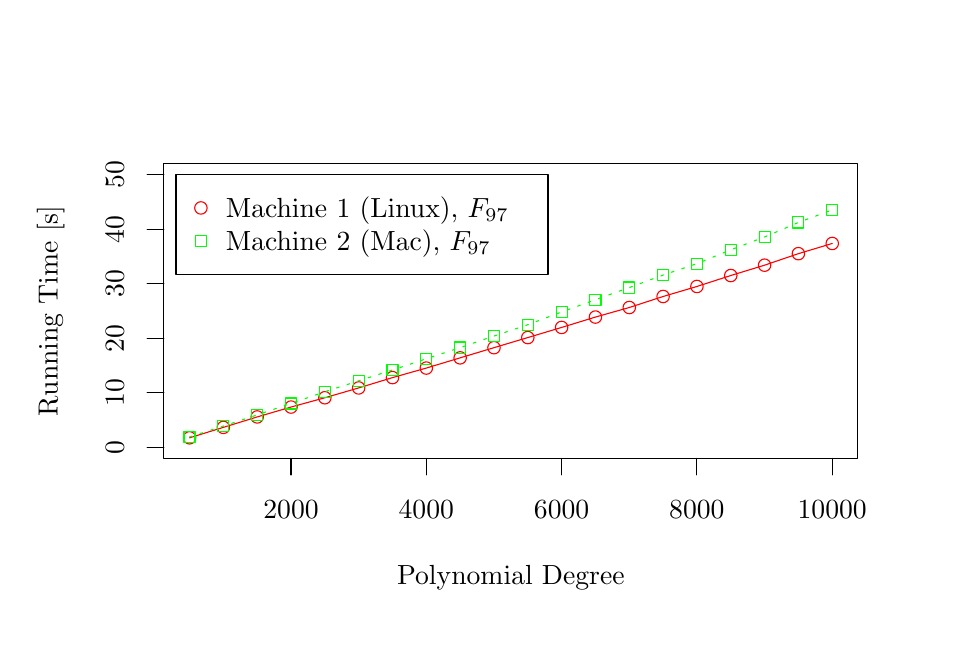
\begin{tikzpicture}[x=1pt,y=1pt]
\definecolor[named]{fillColor}{rgb}{1.00,1.00,1.00}
\path[use as bounding box,fill=fillColor,fill opacity=0.00] (0,0) rectangle (325.21,216.81);
\begin{scope}
\path[clip] ( 49.20, 61.20) rectangle (300.01,167.61);
\definecolor[named]{drawColor}{rgb}{1.00,0.00,0.00}

\path[draw=drawColor,line width= 0.4pt,line join=round,line cap=round] ( 58.49, 68.60) --
	( 70.71, 72.38) --
	( 82.94, 76.15) --
	( 95.16, 79.72) --
	(107.38, 83.08) --
	(119.60, 86.63) --
	(131.83, 90.36) --
	(144.05, 93.81) --
	(156.27, 97.50) --
	(168.50,101.18) --
	(180.72,104.83) --
	(192.94,108.49) --
	(205.16,112.24) --
	(217.39,115.69) --
	(229.61,119.67) --
	(241.83,123.29) --
	(254.06,127.25) --
	(266.28,130.99) --
	(278.50,135.15) --
	(290.73,138.83);

\path[draw=drawColor,line width= 0.4pt,line join=round,line cap=round] ( 58.49, 68.60) circle (  2.25);

\path[draw=drawColor,line width= 0.4pt,line join=round,line cap=round] ( 70.71, 72.38) circle (  2.25);

\path[draw=drawColor,line width= 0.4pt,line join=round,line cap=round] ( 82.94, 76.15) circle (  2.25);

\path[draw=drawColor,line width= 0.4pt,line join=round,line cap=round] ( 95.16, 79.72) circle (  2.25);

\path[draw=drawColor,line width= 0.4pt,line join=round,line cap=round] (107.38, 83.08) circle (  2.25);

\path[draw=drawColor,line width= 0.4pt,line join=round,line cap=round] (119.60, 86.63) circle (  2.25);

\path[draw=drawColor,line width= 0.4pt,line join=round,line cap=round] (131.83, 90.36) circle (  2.25);

\path[draw=drawColor,line width= 0.4pt,line join=round,line cap=round] (144.05, 93.81) circle (  2.25);

\path[draw=drawColor,line width= 0.4pt,line join=round,line cap=round] (156.27, 97.50) circle (  2.25);

\path[draw=drawColor,line width= 0.4pt,line join=round,line cap=round] (168.50,101.18) circle (  2.25);

\path[draw=drawColor,line width= 0.4pt,line join=round,line cap=round] (180.72,104.83) circle (  2.25);

\path[draw=drawColor,line width= 0.4pt,line join=round,line cap=round] (192.94,108.49) circle (  2.25);

\path[draw=drawColor,line width= 0.4pt,line join=round,line cap=round] (205.16,112.24) circle (  2.25);

\path[draw=drawColor,line width= 0.4pt,line join=round,line cap=round] (217.39,115.69) circle (  2.25);

\path[draw=drawColor,line width= 0.4pt,line join=round,line cap=round] (229.61,119.67) circle (  2.25);

\path[draw=drawColor,line width= 0.4pt,line join=round,line cap=round] (241.83,123.29) circle (  2.25);

\path[draw=drawColor,line width= 0.4pt,line join=round,line cap=round] (254.06,127.25) circle (  2.25);

\path[draw=drawColor,line width= 0.4pt,line join=round,line cap=round] (266.28,130.99) circle (  2.25);

\path[draw=drawColor,line width= 0.4pt,line join=round,line cap=round] (278.50,135.15) circle (  2.25);

\path[draw=drawColor,line width= 0.4pt,line join=round,line cap=round] (290.73,138.83) circle (  2.25);
\end{scope}
\begin{scope}
\path[clip] (  0.00,  0.00) rectangle (325.21,216.81);
\definecolor[named]{drawColor}{rgb}{0.00,0.00,0.00}

\path[draw=drawColor,line width= 0.4pt,line join=round,line cap=round] ( 95.16, 61.20) -- (290.73, 61.20);

\path[draw=drawColor,line width= 0.4pt,line join=round,line cap=round] ( 95.16, 61.20) -- ( 95.16, 55.20);

\path[draw=drawColor,line width= 0.4pt,line join=round,line cap=round] (144.05, 61.20) -- (144.05, 55.20);

\path[draw=drawColor,line width= 0.4pt,line join=round,line cap=round] (192.94, 61.20) -- (192.94, 55.20);

\path[draw=drawColor,line width= 0.4pt,line join=round,line cap=round] (241.83, 61.20) -- (241.83, 55.20);

\path[draw=drawColor,line width= 0.4pt,line join=round,line cap=round] (290.73, 61.20) -- (290.73, 55.20);

\node[text=drawColor,anchor=base,inner sep=0pt, outer sep=0pt, scale=  1.00] at ( 95.16, 39.60) {2000};

\node[text=drawColor,anchor=base,inner sep=0pt, outer sep=0pt, scale=  1.00] at (144.05, 39.60) {4000};

\node[text=drawColor,anchor=base,inner sep=0pt, outer sep=0pt, scale=  1.00] at (192.94, 39.60) {6000};

\node[text=drawColor,anchor=base,inner sep=0pt, outer sep=0pt, scale=  1.00] at (241.83, 39.60) {8000};

\node[text=drawColor,anchor=base,inner sep=0pt, outer sep=0pt, scale=  1.00] at (290.73, 39.60) {10000};

\path[draw=drawColor,line width= 0.4pt,line join=round,line cap=round] ( 49.20, 65.14) -- ( 49.20,163.67);

\path[draw=drawColor,line width= 0.4pt,line join=round,line cap=round] ( 49.20, 65.14) -- ( 43.20, 65.14);

\path[draw=drawColor,line width= 0.4pt,line join=round,line cap=round] ( 49.20, 84.85) -- ( 43.20, 84.85);

\path[draw=drawColor,line width= 0.4pt,line join=round,line cap=round] ( 49.20,104.55) -- ( 43.20,104.55);

\path[draw=drawColor,line width= 0.4pt,line join=round,line cap=round] ( 49.20,124.26) -- ( 43.20,124.26);

\path[draw=drawColor,line width= 0.4pt,line join=round,line cap=round] ( 49.20,143.96) -- ( 43.20,143.96);

\path[draw=drawColor,line width= 0.4pt,line join=round,line cap=round] ( 49.20,163.67) -- ( 43.20,163.67);

\node[text=drawColor,rotate= 90.00,anchor=base,inner sep=0pt, outer sep=0pt, scale=  1.00] at ( 34.80, 65.14) {0};

\node[text=drawColor,rotate= 90.00,anchor=base,inner sep=0pt, outer sep=0pt, scale=  1.00] at ( 34.80, 84.85) {10};

\node[text=drawColor,rotate= 90.00,anchor=base,inner sep=0pt, outer sep=0pt, scale=  1.00] at ( 34.80,104.55) {20};

\node[text=drawColor,rotate= 90.00,anchor=base,inner sep=0pt, outer sep=0pt, scale=  1.00] at ( 34.80,124.26) {30};

\node[text=drawColor,rotate= 90.00,anchor=base,inner sep=0pt, outer sep=0pt, scale=  1.00] at ( 34.80,143.96) {40};

\node[text=drawColor,rotate= 90.00,anchor=base,inner sep=0pt, outer sep=0pt, scale=  1.00] at ( 34.80,163.67) {50};

\path[draw=drawColor,line width= 0.4pt,line join=round,line cap=round] ( 49.20, 61.20) --
	(300.01, 61.20) --
	(300.01,167.61) --
	( 49.20,167.61) --
	( 49.20, 61.20);
\end{scope}
\begin{scope}
\path[clip] (  0.00,  0.00) rectangle (325.21,216.81);
\definecolor[named]{drawColor}{rgb}{0.00,0.00,0.00}

\node[text=drawColor,anchor=base,inner sep=0pt, outer sep=0pt, scale=  1.00] at (174.61, 15.60) {Polynomial Degree};

\node[text=drawColor,rotate= 90.00,anchor=base,inner sep=0pt, outer sep=0pt, scale=  1.00] at ( 10.80,114.41) {Running Time [s]};
\end{scope}
\begin{scope}
\path[clip] ( 49.20, 61.20) rectangle (300.01,167.61);
\definecolor[named]{drawColor}{rgb}{0.00,1.00,0.00}

\path[draw=drawColor,line width= 0.4pt,dash pattern=on 1pt off 3pt ,line join=round,line cap=round] ( 58.49, 68.91) --
	( 70.71, 72.84) --
	( 82.94, 76.89) --
	( 95.16, 81.02) --
	(107.38, 85.24) --
	(119.60, 89.21) --
	(131.83, 93.11) --
	(144.05, 97.16) --
	(156.27,101.21) --
	(168.50,105.37) --
	(180.72,109.47) --
	(192.94,114.08) --
	(205.16,118.51) --
	(217.39,122.90) --
	(229.61,127.41) --
	(241.83,131.54) --
	(254.06,136.54) --
	(266.28,141.17) --
	(278.50,146.42) --
	(290.73,150.96);

\path[draw=drawColor,line width= 0.4pt,line join=round,line cap=round] ( 56.50, 66.92) rectangle ( 60.48, 70.91);

\path[draw=drawColor,line width= 0.4pt,line join=round,line cap=round] ( 68.72, 70.84) rectangle ( 72.71, 74.83);

\path[draw=drawColor,line width= 0.4pt,line join=round,line cap=round] ( 80.94, 74.89) rectangle ( 84.93, 78.88);

\path[draw=drawColor,line width= 0.4pt,line join=round,line cap=round] ( 93.16, 79.02) rectangle ( 97.15, 83.01);

\path[draw=drawColor,line width= 0.4pt,line join=round,line cap=round] (105.39, 83.24) rectangle (109.38, 87.23);

\path[draw=drawColor,line width= 0.4pt,line join=round,line cap=round] (117.61, 87.22) rectangle (121.60, 91.21);

\path[draw=drawColor,line width= 0.4pt,line join=round,line cap=round] (129.83, 91.12) rectangle (133.82, 95.11);

\path[draw=drawColor,line width= 0.4pt,line join=round,line cap=round] (142.06, 95.16) rectangle (146.04, 99.15);

\path[draw=drawColor,line width= 0.4pt,line join=round,line cap=round] (154.28, 99.22) rectangle (158.27,103.21);

\path[draw=drawColor,line width= 0.4pt,line join=round,line cap=round] (166.50,103.38) rectangle (170.49,107.37);

\path[draw=drawColor,line width= 0.4pt,line join=round,line cap=round] (178.72,107.48) rectangle (182.71,111.47);

\path[draw=drawColor,line width= 0.4pt,line join=round,line cap=round] (190.95,112.09) rectangle (194.94,116.07);

\path[draw=drawColor,line width= 0.4pt,line join=round,line cap=round] (203.17,116.52) rectangle (207.16,120.50);

\path[draw=drawColor,line width= 0.4pt,line join=round,line cap=round] (215.39,120.91) rectangle (219.38,124.90);

\path[draw=drawColor,line width= 0.4pt,line join=round,line cap=round] (227.62,125.42) rectangle (231.60,129.41);

\path[draw=drawColor,line width= 0.4pt,line join=round,line cap=round] (239.84,129.54) rectangle (243.83,133.53);

\path[draw=drawColor,line width= 0.4pt,line join=round,line cap=round] (252.06,134.54) rectangle (256.05,138.53);

\path[draw=drawColor,line width= 0.4pt,line join=round,line cap=round] (264.29,139.18) rectangle (268.27,143.16);

\path[draw=drawColor,line width= 0.4pt,line join=round,line cap=round] (276.51,144.43) rectangle (280.50,148.42);

\path[draw=drawColor,line width= 0.4pt,line join=round,line cap=round] (288.73,148.97) rectangle (292.72,152.96);
\definecolor[named]{drawColor}{rgb}{0.00,0.00,0.00}

\path[draw=drawColor,line width= 0.4pt,line join=round,line cap=round] ( 53.60,163.67) rectangle (188.02,127.67);
\definecolor[named]{drawColor}{rgb}{1.00,0.00,0.00}

\path[draw=drawColor,line width= 0.4pt,line join=round,line cap=round] ( 62.60,151.67) circle (  2.25);
\definecolor[named]{drawColor}{rgb}{0.00,1.00,0.00}

\path[draw=drawColor,line width= 0.4pt,line join=round,line cap=round] ( 60.61,137.67) rectangle ( 64.59,141.66);
\definecolor[named]{drawColor}{rgb}{0.00,0.00,0.00}

\node[text=drawColor,anchor=base west,inner sep=0pt, outer sep=0pt, scale=  1.00] at ( 71.60,148.23) {Machine 1 (Linux), $\mathbb{F}_{97}\ \ \ $};

\node[text=drawColor,anchor=base west,inner sep=0pt, outer sep=0pt, scale=  1.00] at ( 71.60,136.23) {Machine 2 (Mac), $\mathbb{F}_{97}$};
\end{scope}
\end{tikzpicture}
